\chapter{Lecture 3 - Carnot Cycle and Exergy Overview}
\label{ch:ch3}
\section{Objectives}
The objectives of this lecture are:
\begin{itemize}
\item Describe the Carnot Cycle
\item Review the Simple Ideal Rankine Cycle in context of a Carnot Cycle
\item Introduce exergy and provide related definitions.
\end{itemize}

\section{The Carnot Cycle}
\index{Carnot Cycle}
\newthought{The Carnot cycle is} an idealized heat engine that you should have learned about in a basic thermodynamics class or from a reference text.\cite{moran2010fundamentals}  It is idealized in the sense that it represents the most efficient possible heat engine working between two (high and low temperature) thermal reservoirs.  A temperature-entropy plot of the cycle is shown in figure \ref{fig:CarnotCycle} and consists of four processes:

\begin{marginfigure}
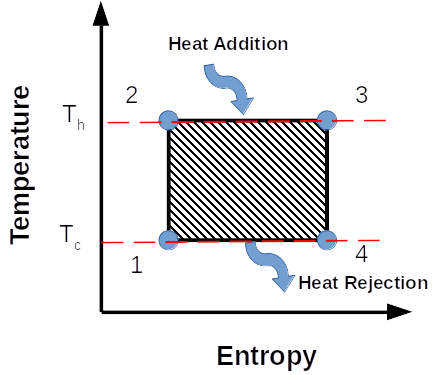
\includegraphics{Carnot_cycle_sketch.png}
\caption{Temperature-Entropy plot of a Carnot cycle.}
\label{fig:CarnotCycle}
\end{marginfigure}

\begin{enumerate}
\item isentropic compression $1 \rightarrow 2$
\item isothermal heat addition $2 \rightarrow 3$
\item isentropic expansion $3 \rightarrow 4$
\item isothermal heat rejection $4 \rightarrow 1$

\end{enumerate}

The thermal efficiency of this cycle can be shown to be a function of the absolute temperature of the high temperature reservoir $\left(T_h\right)$ and the absolute temperature of the low temperature reservoir $\left(T_c\right)$.  

$$ \eta_{\text{Carnot}} = 1 - \frac{T_c}{T_h}$$ \index{efficiency, Carnot}

Note that as $T_c$ decreases or as $T_h$ increases, the Carnot efficiency increases.  Since both reservoir absolute temperatures are non-negative, and $T_h > T_c$, the Carnot efficiency can be no greater than 1 and achieves that only for $T_c=0$ or as $T_h \rightarrow \infty$.  

\newthought{The following concepts} should be emphasized:
\begin{enumerate}
\item No heat engine can convert all heat input to work; and
\item A Carnot cycle is a heat engine that produces the maximum possible efficiency for any heat engine operating between a given fixed hot and cold temperature reservoir.
\end{enumerate}

All of the processes of the Carnot Cycle are reversible and the work-in and work-out of process 1 and 3 are isentropic.  The heat-in and heat-out of process 2 and 4 are reversible because the heat is transferred isothermally.\marginnote[-4cm]{\textbf{Note: }It is not evident from the temperature-entropy diagram, but the isothermal heat transfer processes in a Carnot cycle also must take place across an infinitesimal temperature gradient.  We know from the laws of heat transfer that heat flows from high temperature to low temperature and the rate of heat transfer is proportional to:
\begin{enumerate}
\item the size of the heat transfer surface, 
\item the temperature difference, and 
\item some material property characterizing how ``well'' heat is transferred.  
\end{enumerate}
In order to transfer energy across an infinitesimal temperature gradient, the material must have arbitrarily good heat transfer properties, or the heat transfer surface must be arbitrarily large.  We will dismiss these practical complications for the time being and simply move forward. }

\section{Simple Ideal Rankine Cycle - Revisited}
\newthought{Consider again the} Simple Ideal Rankine cycle operating between the maximum pressure of 838 psia and minimum pressure of 1.5 psia.  A schematic temperature-entropy diagram of this process is shown below.

\begin{figure}
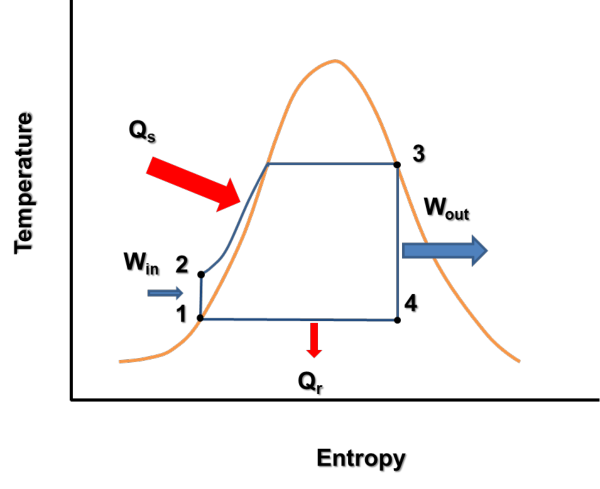
\includegraphics{simple_ideal_rankine_TS.pdf}
\caption{Temperature-Entropy plot of a simple, ideal, Rankine cycle.}
\label{fig:simple_rankine_TS_2}
\end{figure} 

From the example in Lecture 1, we know that the thermal efficiency is 35.1 percent and the net specific work is 390.3 BTU/lbm.  What is the Carnot efficiency of this cycle?
\begin{itemize}
\item To calculate the Carnot efficiency, we need the temperature of the hot and cold reservoirs respectively.
\item If we take $T_h$ to be the saturation temperature at 838 psia, we find that it is approximately 524 $^{\circ}$F; this corresponds to 984 R.\sidenote{If we're analyzing an AP1000 PWR energy conversion cycle, a better choice for $T_h$ would be the hot-leg temperature which is approximately 610 $^{\circ}$F.  We will come back to this in a future lecture.} 
\item If we take $T_c$ to be the condenser temperature (for heat rejection from state point 4 to 1), which is equal to the saturation pressure at 1.5 psia, we find that it is approximately 116 $^{\circ}$F; this corresponds to 576 R.\sidenote{Again, a better choice for $T_c$ for the AP1000 would be the inlet temperature of cooling water to the condenser which we might conservatively take to be 91 $^{\circ}$F.}
\item Thus the Carnot efficiency is: $\eta_{\text{C}} = 1 - \sfrac{576}{984} = 0.415$; or 41.5 percent.  
\end{itemize}

Consider the heat addition $(Q_s)$ from state points 2 to 3; unlike the Carnot cycle, the heat transfer does not occur isothermally.  Significant irreversibilities exist in this process.  Although the heat rejected in the process from state point 4 to 1 does occur at constant temperature, in practice the heat is rejected to an external heat sink across a finite temperature difference. This also is a source of irreversibility although it is not evident from the temperature-entropy diagram.  

\newthought{Suppose we modified} the Rankine Cycle above to make it \emph{more like} a Carnot cycle.  We could reject heat only to state point 1' in Figure \ref{fig:simple_rankine_TS_carnot} and apply work to isentropically compress the mixture until it became a saturated liquid at 838 psia, state point 2'.  What would the thermal efficiency be for that cycle?

\begin{marginfigure}
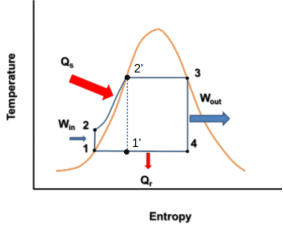
\includegraphics{simple_ideal_rankine_TS_carnot.pdf}
\caption{Temperature-Entropy plot of a modified Rankine cycle.}
\label{fig:simple_rankine_TS_carnot}
\end{marginfigure} 

The answer is 41.5 percent just like the Carnot cycle.  You would also find that the net specific work for the cycle is somewhat reduced.  Is that what you expect?  Again, the answer should be ``yes''; by changing state points 1 and 2 we reduced the area contained within the T-S diagram and that corresponds with reduced net specific work.

\index{Exergy}
\section{Exergy Analysis - Basic Definitions}
In order to analyze quantitatively the extent to which a cycle has reversibility we will need to perform an \emph{Exergy Analysis}.\marginnote{The course textbook does an \emph{irreversibility} analysis which is equivalent.}

\subsection{Definitions}
The following definitions are provided below:
\begin{itemize}
\item \emph{Exergy} is the maximum theoretically obtainable work that can be extracted from a working fluid as it comes into equilibrium with the environment.\marginnote[-1.5cm]{\textbf{Note: } exergy is defined for a working fluid only \emph{relative} to the environment.  Working fluid of a given state will have a different exergy if environmental temperature or pressure goes up or down.}

\index{Dead state}
\item \emph{Dead state} is a state in which a working fluid is at rest relative to the environment.  The dead state will normally be characterized by dead state temperature $(T_o)$ and dead state pressure $(P_o)$.

\index{Exergy, specific flow}
\item \emph{Specific Flow Exergy} ($e_f$) is an intrinsic thermodynamic variable quantifying the ability of a working fluid to do work.  It is calculated relative to the dead state as follows:
$$e_f = h - h_o - T_o(s - s_o) + \frac{V^2}{2} + gz$$
where $h$ and $s$ are the enthalpy and entropy of the working fluid; $h_o$ and $s_o$ are the enthalpy and entropy at the dead state temperature and pressure; $T_o$ is the dead state temperature; and $\sfrac{V^2}{2}$ and $gz$ represent the kinetic and potential energy respectively of the fluid.\sidenote{Unless otherwise noted, changes in kinetic and potential energy will be neglected in this class so, for calculations of $e_f$, those terms are excluded.}

\end{itemize}

\index{Exergy Balance}
\subsection{Exergy Balance}
\newthought{Unlike energy,} exergy is not conserved.  One can think of exergy like energy: we pass exergy in from a high energy source like the primary coolant of a PWR; we convert some of that exergy to work and some that is left over we have to reject to the environment.  But unlike energy, exergy can be destroyed. Exergy can also be lost through other means like heat transfer to the surrounding medium.\sidenote[][-1cm]{For example: steam piping passing through the engineroom of a submarine is hot; despite its lagging, it transfers some energy to the surrounding environment.  This is a loss of exergy that can be taken into account.}

We want to account for exergy in much the same way that we account for energy.  In words, this accounting balance looks like this:

$$\text{Exergy in} - \text{Exergy out} = \text{Exergy xfer by heat} + \text{Exergy xfer by work} + \text{Exergy Destroyed}$$

In equation form this translates as follows:

$$\sum_i \dot{m}_i e_{f_i} - \sum_e \dot{m}_e e_{f_e} = \sum_j \left(1-\frac{T_o}{T_j} \right)\dot{Q_j}+\dot{W} + \dot{E}_d$$
The terms are interpreted as follows:
\begin{itemize}
\item $\sum_i\dot{m}_i e_{f_i}$ is the sum of all flow exergy going \emph{in} to a particular process.  The variable $i$ corresponds to all of the inflows; $\dot{m}_i$ is the mass flow rate for each in-flow and $e_{f_i}$ is the specific flow exergy for each inflow.
\item $\sum_e \dot{m}_e e_{f_e}$ has the same meaning but for all flows \emph{exiting} a particular process.
\item $\sum_j \left(1-\sfrac{T_o}{T_j} \right)\dot{Q_j}$ is exergy transfer through heat. The variable $j$ enumerates all of the exit points for exergy transfer through heat for the system. $\dot{Q}_j$ is the corresponding rate of heat loss, $T_j$ is the temperature at which this heat is lost, and $T_o$ is the dead state temperature.
\item $\dot{W}$ is the rate of exergy transfer through work.  Any process that does work (e.g. turbine, pump, compressor) transfers exergy out of (turbine) or into (pump or compressor) the working fluid.
\item $\dot{E}_d$ is the rate of exergy destruction.  This should be interpreted as the rate at which exergy is lost due to irreversibilities.  Any non-reversible process will have positive exergy destruction.\sidenote{Exergy destruction rate for a process should \emph{never} be negative.  If your calculations show a negative exergy destruction rate (other than rounding errors near zero) for any process you have somehow violated the Second Law of Thermodynamics.  You need to stop and find the error before moving forward.}
\end{itemize}




